\documentclass[]{article}
\usepackage{lmodern}
\usepackage{amssymb,amsmath}
\usepackage{ifxetex,ifluatex}
\usepackage{fixltx2e} % provides \textsubscript
\ifnum 0\ifxetex 1\fi\ifluatex 1\fi=0 % if pdftex
  \usepackage[T1]{fontenc}
  \usepackage[utf8]{inputenc}
\else % if luatex or xelatex
  \ifxetex
    \usepackage{mathspec}
  \else
    \usepackage{fontspec}
  \fi
  \defaultfontfeatures{Ligatures=TeX,Scale=MatchLowercase}
\fi
% use upquote if available, for straight quotes in verbatim environments
\IfFileExists{upquote.sty}{\usepackage{upquote}}{}
% use microtype if available
\IfFileExists{microtype.sty}{%
\usepackage{microtype}
\UseMicrotypeSet[protrusion]{basicmath} % disable protrusion for tt fonts
}{}
\usepackage[margin=1in]{geometry}
\usepackage{hyperref}
\hypersetup{unicode=true,
            pdftitle={Assignment 10},
            pdfauthor={Reid Ginoza},
            pdfborder={0 0 0},
            breaklinks=true}
\urlstyle{same}  % don't use monospace font for urls
\usepackage{color}
\usepackage{fancyvrb}
\newcommand{\VerbBar}{|}
\newcommand{\VERB}{\Verb[commandchars=\\\{\}]}
\DefineVerbatimEnvironment{Highlighting}{Verbatim}{commandchars=\\\{\}}
% Add ',fontsize=\small' for more characters per line
\usepackage{framed}
\definecolor{shadecolor}{RGB}{248,248,248}
\newenvironment{Shaded}{\begin{snugshade}}{\end{snugshade}}
\newcommand{\AlertTok}[1]{\textcolor[rgb]{0.94,0.16,0.16}{#1}}
\newcommand{\AnnotationTok}[1]{\textcolor[rgb]{0.56,0.35,0.01}{\textbf{\textit{#1}}}}
\newcommand{\AttributeTok}[1]{\textcolor[rgb]{0.77,0.63,0.00}{#1}}
\newcommand{\BaseNTok}[1]{\textcolor[rgb]{0.00,0.00,0.81}{#1}}
\newcommand{\BuiltInTok}[1]{#1}
\newcommand{\CharTok}[1]{\textcolor[rgb]{0.31,0.60,0.02}{#1}}
\newcommand{\CommentTok}[1]{\textcolor[rgb]{0.56,0.35,0.01}{\textit{#1}}}
\newcommand{\CommentVarTok}[1]{\textcolor[rgb]{0.56,0.35,0.01}{\textbf{\textit{#1}}}}
\newcommand{\ConstantTok}[1]{\textcolor[rgb]{0.00,0.00,0.00}{#1}}
\newcommand{\ControlFlowTok}[1]{\textcolor[rgb]{0.13,0.29,0.53}{\textbf{#1}}}
\newcommand{\DataTypeTok}[1]{\textcolor[rgb]{0.13,0.29,0.53}{#1}}
\newcommand{\DecValTok}[1]{\textcolor[rgb]{0.00,0.00,0.81}{#1}}
\newcommand{\DocumentationTok}[1]{\textcolor[rgb]{0.56,0.35,0.01}{\textbf{\textit{#1}}}}
\newcommand{\ErrorTok}[1]{\textcolor[rgb]{0.64,0.00,0.00}{\textbf{#1}}}
\newcommand{\ExtensionTok}[1]{#1}
\newcommand{\FloatTok}[1]{\textcolor[rgb]{0.00,0.00,0.81}{#1}}
\newcommand{\FunctionTok}[1]{\textcolor[rgb]{0.00,0.00,0.00}{#1}}
\newcommand{\ImportTok}[1]{#1}
\newcommand{\InformationTok}[1]{\textcolor[rgb]{0.56,0.35,0.01}{\textbf{\textit{#1}}}}
\newcommand{\KeywordTok}[1]{\textcolor[rgb]{0.13,0.29,0.53}{\textbf{#1}}}
\newcommand{\NormalTok}[1]{#1}
\newcommand{\OperatorTok}[1]{\textcolor[rgb]{0.81,0.36,0.00}{\textbf{#1}}}
\newcommand{\OtherTok}[1]{\textcolor[rgb]{0.56,0.35,0.01}{#1}}
\newcommand{\PreprocessorTok}[1]{\textcolor[rgb]{0.56,0.35,0.01}{\textit{#1}}}
\newcommand{\RegionMarkerTok}[1]{#1}
\newcommand{\SpecialCharTok}[1]{\textcolor[rgb]{0.00,0.00,0.00}{#1}}
\newcommand{\SpecialStringTok}[1]{\textcolor[rgb]{0.31,0.60,0.02}{#1}}
\newcommand{\StringTok}[1]{\textcolor[rgb]{0.31,0.60,0.02}{#1}}
\newcommand{\VariableTok}[1]{\textcolor[rgb]{0.00,0.00,0.00}{#1}}
\newcommand{\VerbatimStringTok}[1]{\textcolor[rgb]{0.31,0.60,0.02}{#1}}
\newcommand{\WarningTok}[1]{\textcolor[rgb]{0.56,0.35,0.01}{\textbf{\textit{#1}}}}
\usepackage{graphicx,grffile}
\makeatletter
\def\maxwidth{\ifdim\Gin@nat@width>\linewidth\linewidth\else\Gin@nat@width\fi}
\def\maxheight{\ifdim\Gin@nat@height>\textheight\textheight\else\Gin@nat@height\fi}
\makeatother
% Scale images if necessary, so that they will not overflow the page
% margins by default, and it is still possible to overwrite the defaults
% using explicit options in \includegraphics[width, height, ...]{}
\setkeys{Gin}{width=\maxwidth,height=\maxheight,keepaspectratio}
\IfFileExists{parskip.sty}{%
\usepackage{parskip}
}{% else
\setlength{\parindent}{0pt}
\setlength{\parskip}{6pt plus 2pt minus 1pt}
}
\setlength{\emergencystretch}{3em}  % prevent overfull lines
\providecommand{\tightlist}{%
  \setlength{\itemsep}{0pt}\setlength{\parskip}{0pt}}
\setcounter{secnumdepth}{0}
% Redefines (sub)paragraphs to behave more like sections
\ifx\paragraph\undefined\else
\let\oldparagraph\paragraph
\renewcommand{\paragraph}[1]{\oldparagraph{#1}\mbox{}}
\fi
\ifx\subparagraph\undefined\else
\let\oldsubparagraph\subparagraph
\renewcommand{\subparagraph}[1]{\oldsubparagraph{#1}\mbox{}}
\fi

%%% Use protect on footnotes to avoid problems with footnotes in titles
\let\rmarkdownfootnote\footnote%
\def\footnote{\protect\rmarkdownfootnote}

%%% Change title format to be more compact
\usepackage{titling}

% Create subtitle command for use in maketitle
\providecommand{\subtitle}[1]{
  \posttitle{
    \begin{center}\large#1\end{center}
    }
}

\setlength{\droptitle}{-2em}

  \title{Assignment 10}
    \pretitle{\vspace{\droptitle}\centering\huge}
  \posttitle{\par}
    \author{Reid Ginoza}
    \preauthor{\centering\large\emph}
  \postauthor{\par}
      \predate{\centering\large\emph}
  \postdate{\par}
    \date{4/19/2020}

\newcommand{\D}{\mathrm{d}}
\DeclareMathOperator*{\argmin}{arg\,min}

\begin{document}
\maketitle

\hypertarget{ornstein-uhlenbeck-maximum-likelihood-estimate}{%
\section{Ornstein-Uhlenbeck Maximum Likelihood
Estimate}\label{ornstein-uhlenbeck-maximum-likelihood-estimate}}

The analytical problem is to derive the maximum likehood estimate for
the Ornstein-Uhlenbeck process. This is Exercise 11.4 from (Särkkä and
Solin 2019), and we are guided by the authors' instructions. The
Ornstein-Uhlenbeck process is defined as follows: \begin{equation}
\mathrm{d}x = - \lambda x \mathrm{d}t + \mathrm{d}\beta, \quad x \left( 0 \right) = x_0,
\end{equation} where \(\lambda\) is unknown and \(\beta\) has an unknown
diffiusion constant \(q\). Thus, we define the unknown parameters as the
vector \(\theta = \left(\lambda, q\right)\). The authors also previously
provided the transition density: \begin{equation}
p\left( x\left( t + \Delta t \right) \vert x \left( t \right) \right) =
\mathrm{N} \left( x\left( t + \Delta t \right) \vert \exp{\left( - \lambda \Delta t \right)} x \left( t \right),
\dfrac{q}{2 \lambda} \left[ 1 - \exp{\left( - 2 \lambda \Delta t \right)} \right] \right)
\end{equation}

The negative log-likelihood is: \begin{equation}
\ell(\lambda, q) = \sum_{k=0}^{T-1} \left[ \dfrac{1}{2} \log{\left( 2 \pi \dfrac{q}{2\lambda} \left[ 1 - \exp{\left( - 2 \lambda \Delta t \right)} \right] \right)}
+ \dfrac{\lambda}{q \left[ 1 - \exp{\left( - 2 \lambda \Delta t \right)} \right]}
\left( x(t_{k+1}) - \exp{\left( - \lambda \Delta t \right)} x(t_k) \right)^2 \right]
\end{equation} and using this change of variables: \begin{align}
a &= \exp{\left( - \lambda \Delta t \right)}\\
\Sigma &= \dfrac{q}{2 \lambda} \left[ 1 - \exp{\left( - 2 \lambda \Delta t \right)} \right]
\end{align} we arrive at: \begin{equation}
\ell (a, \Sigma) = \sum_{k=0}^{T-1} \left[ \dfrac{1}{2} \log{\left( 2 \pi \Sigma \right)} 
+ \dfrac{1}{2 \Sigma} \left( x(t_{k+1}) - a x(t_k) \right)^2 \right]
\end{equation}

To find the maximum likelihood, we find where \(\ell\) has a gradient of
0. \begin{align}
\dfrac{\partial \ell}{\partial a} &=
- \dfrac{1}{\Sigma} \sum_{k=0}^{T-1} \left( x(t_{k+1}) - a x(t_k) \right) x(t_k) = 0\\
\implies 0 &= \sum_{k=0}^{T-1} x(t_{k+1})x(t_k)  - a \sum_{k=1}^{T-1} \left(x(t_k)\right)^2\\
\implies  a_{\mathrm{ML}} &= \dfrac{\sum_{k=0}^{T-1} x(t_{k+1})x(t_k)}{\sum_{k=1}^{T-1} \left(x(t_k)\right)^2}\\
&\, \\
\dfrac{\partial \ell}{\partial \Sigma} &=
\sum_{k=0}^{T-1} \left[ \dfrac{1}{2 \Sigma} - \dfrac{1}{2 \Sigma^2} \left( x(t_{k+1}) - a x(t_k) \right)^2 \right] = 0\\
0 &= \dfrac{T}{2 \Sigma} - \dfrac{1}{2 \Sigma^2} \sum_{k=0}^{T-1} \left( x(t_{k+1}) - a x(t_k) \right)^2\\
\implies \dfrac{T}{2 \Sigma} &= \dfrac{1}{2 \Sigma^2} \sum_{k=0}^{T-1} \left( x(t_{k+1}) - a x(t_k) \right)^2\\
\implies T \Sigma &= \sum_{k=0}^{T-1} \left( x(t_{k+1}) - a x(t_k) \right)^2\\
\implies \Sigma_{\mathrm{ML}} &= \dfrac{1}{T} \sum_{k=0}^{T-1} \left( x(t_{k+1}) - a_{\mathrm{ML}} x(t_k) \right)^2
\end{align}

And to reverse the change of variables, we used: \begin{align}
a_{\mathrm{ML}} &= \exp{\left( - \lambda_{\mathrm{ML}} \Delta t \right)}\\
\Sigma_{\mathrm{ML}} &= \dfrac{q_{\mathrm{ML}}}{2 \lambda} \left[ 1 - \exp{\left( - 2 \lambda_{\mathrm{ML}} \Delta t \right)} \right]
\end{align}

which gives \begin{align}
a_{\mathrm{ML}} &= \dfrac{\sum_{k=0}^{T-1} x(t_{k+1})x(t_k)}{\sum_{k=1}^{T-1} \left(x(t_k)\right)^2}\\
\exp{\left( - \lambda_{\mathrm{ML}} \Delta t \right)} &= \dfrac{\sum_{k=0}^{T-1} x(t_{k+1})x(t_k)}{\sum_{k=1}^{T-1} \left(x(t_k)\right)^2}\\
\lambda_{\mathrm{ML}} &= - \dfrac{1}{\Delta t} \log{\left[ \dfrac{\sum_{k=0}^{T-1} x(t_{k+1})x(t_k)}{\sum_{k=1}^{T-1} \left(x(t_k)\right)^2} \right]}\\
&\, \\
\Sigma_{\mathrm{ML}} &= \dfrac{1}{T} \sum_{k=0}^{T-1} \left( x(t_{k+1}) - a_{\mathrm{ML}} x(t_k) \right)^2\\
\dfrac{q_{\mathrm{ML}}}{2 \lambda} \left[ 1 - \exp{\left( - 2 \lambda_{\mathrm{ML}} \Delta t \right)} \right]
&= \dfrac{1}{T} \sum_{k=0}^{T-1} \left( x(t_{k+1}) - a_{\mathrm{ML}} x(t_k) \right)^2\\
\implies q_{\mathrm{ML}} &= \dfrac{2 \lambda_{\mathrm{ML}}}{T \left[ 1 - \exp{\left( - 2 \lambda_{\mathrm{ML}} \Delta t \right)} \right]}
\sum_{k=0}^{T-1} \left( x(t_{k+1}) - \exp{\left( - \lambda_{\mathrm{ML}} \Delta t \right)} x(t_k) \right)^2
\end{align}

\hypertarget{computational-problem}{%
\section{Computational Problem}\label{computational-problem}}

This is problem 11.9 from (Särkkä and Solin 2019) and concerns a model
where two parameters \(\theta_1\) and \(\theta_2\) are unknown:
\begin{equation}
\mathrm{d}x = \theta_1 \sin{\left( x - \theta_2 \right)} + \mathrm{d}\beta, \quad x(0) = x_0,
\end{equation} where \(\beta\) is a standard Brownian motion (i.e.~the
diffusion coeffient \(q=1\)).

I was restricted in the number of time steps based on the product
required to calculate the negative log-likihood. I also only sampled one
path. As a result, the numerical method did not find the true parameters
very well.

First, I'll show the Euler-Maruyama approximation of the true function.
Then I will show the optimal parameters based on the maximum likelihood
method based on one sample path.

\begin{Shaded}
\begin{Highlighting}[]
\ImportTok{import}\NormalTok{ numpy }\ImportTok{as}\NormalTok{ np}
\ImportTok{from}\NormalTok{ matplotlib }\ImportTok{import}\NormalTok{ pyplot }\ImportTok{as}\NormalTok{ plt}
\ImportTok{from}\NormalTok{ scipy.optimize }\ImportTok{import}\NormalTok{ minimize}
\ImportTok{from}\NormalTok{ scipy.stats }\ImportTok{import}\NormalTok{ norm}


\CommentTok{# -- Plotting Tools --}
\KeywordTok{def}\NormalTok{ low_buff(y_values):}
\NormalTok{    span }\OperatorTok{=}\NormalTok{ y_values.}\BuiltInTok{max}\NormalTok{() }\OperatorTok{-}\NormalTok{ y_values.}\BuiltInTok{min}\NormalTok{()}
    \ControlFlowTok{return}\NormalTok{ y_values.}\BuiltInTok{min}\NormalTok{() }\OperatorTok{-} \FloatTok{0.1} \OperatorTok{*}\NormalTok{ span}


\KeywordTok{def}\NormalTok{ plot_on_axis(ax, time, pos, cols, title, color_map, with_mean}\OperatorTok{=}\VariableTok{False}\NormalTok{):}
    \ControlFlowTok{for}\NormalTok{ idx, col }\KeywordTok{in} \BuiltInTok{enumerate}\NormalTok{(cols):}
\NormalTok{        ax.plot(time, pos[:, col], c}\OperatorTok{=}\NormalTok{color_map(idx), alpha}\OperatorTok{=}\FloatTok{0.5}\NormalTok{)}
\NormalTok{    ax.set_title(title)}
    \ControlFlowTok{if}\NormalTok{ with_mean:}
\NormalTok{        ax.plot(time, pos.mean(axis}\OperatorTok{=}\DecValTok{1}\NormalTok{), color}\OperatorTok{=}\StringTok{'black'}\NormalTok{,}
\NormalTok{            label}\OperatorTok{=}\VerbatimStringTok{r'Sample Mean $(n=}\SpecialCharTok{\{\}}\VerbatimStringTok{)$'}\NormalTok{.}\BuiltInTok{format}\NormalTok{(pos.shape[}\DecValTok{1}\NormalTok{]), linewidth}\OperatorTok{=}\DecValTok{2}\NormalTok{)}
\NormalTok{        ax.plot(time, pos.mean(axis}\OperatorTok{=}\DecValTok{1}\NormalTok{) }\OperatorTok{+} \DecValTok{2}\OperatorTok{*}\NormalTok{ pos.std(axis}\OperatorTok{=}\DecValTok{1}\NormalTok{), color}\OperatorTok{=}\StringTok{'black'}\NormalTok{,}
\NormalTok{                linestyle}\OperatorTok{=}\StringTok{'dashed'}\NormalTok{)}
\NormalTok{        ax.plot(time, pos.mean(axis}\OperatorTok{=}\DecValTok{1}\NormalTok{) }\OperatorTok{-} \DecValTok{2}\OperatorTok{*}\NormalTok{ pos.std(axis}\OperatorTok{=}\DecValTok{1}\NormalTok{), color}\OperatorTok{=}\StringTok{'black'}\NormalTok{,}
\NormalTok{                linestyle}\OperatorTok{=}\StringTok{'dashed'}\NormalTok{, label}\OperatorTok{=}\StringTok{'Sample Two Std. Dev.'}\NormalTok{)}
\NormalTok{        ax.legend()}


\CommentTok{# -- Brownian Motion --}
\KeywordTok{def}\NormalTok{ multiple_brownian_motion(end_time}\OperatorTok{=}\FloatTok{1.}\NormalTok{, num_tsteps}\OperatorTok{=}\DecValTok{500}\NormalTok{, n_trials}\OperatorTok{=}\DecValTok{1000}\NormalTok{):}
    \CommentTok{"""Creates multiple 1-D Brownian motion with time as the row index and}
\CommentTok{    each column as a separate path of Brownian motion.}

\CommentTok{    This assumes that all Brownian motion starts at 0. Currently only}
\CommentTok{    implements one-dimensional Brownian motion. This also assumes all}
\CommentTok{    step sizes are the same size.}

\CommentTok{    The steps of Brownian motion, ``dw``, are modeled with a Gaussian}
\CommentTok{    distribution with mean 0 and variance ``sqrt(dt)``, where ``dt``}
\CommentTok{    is the constant time step size.}

\CommentTok{    Parameters}
\CommentTok{    ----------}
\CommentTok{    end_time : float}

\CommentTok{    num_tsteps : int}
\CommentTok{        The number of steps to take. Will calculate the step}
\CommentTok{        size dt internally. The number of rows in the output of}
\CommentTok{        Brownian motion will be num_tsteps + 1.}

\CommentTok{    n_trials : int}
\CommentTok{        The number of sample paths to create. This will be the number}
\CommentTok{        of columns in the output.}

\CommentTok{    Returns}
\CommentTok{    -------}
\CommentTok{    t : ndarray}
\CommentTok{        One-dimensional time ndarray from 0 to ``end_time`` with}
\CommentTok{        shape (``num_tsteps``+1,)}

\CommentTok{    w : ndarray}
\CommentTok{        Two-dimensional ndarray representing ``n_trials`` number of}
\CommentTok{        sample paths of one-dimensional Brownian motion.}
\CommentTok{        This will be of shape (``num_tsteps``+1, ``n_trials``).}

\CommentTok{    dt : float}
\CommentTok{        The value indicating the step size of t. This is only implemented}
\CommentTok{        with constant step size.}

\CommentTok{    dw : ndarray}
\CommentTok{        Two-dimensional ndarray representing the steps of Brownian motion.}
\CommentTok{        The first row is all zeros. Each i-th row of ``dw``, ie. dw[i, :]}
\CommentTok{        indicates the change in ``w`` from w[i-1, :] to w[i, :]}
\CommentTok{        This will be the same shape as ``w``, (``num_tsteps``+1, ``n_trials``).}

\CommentTok{    """}

\NormalTok{    dt }\OperatorTok{=}\NormalTok{ (end_time }\OperatorTok{-} \DecValTok{0}\NormalTok{) }\OperatorTok{/}\NormalTok{ num_tsteps}
\NormalTok{    dw }\OperatorTok{=}\NormalTok{ np.random.normal(scale}\OperatorTok{=}\NormalTok{np.sqrt(dt), size}\OperatorTok{=}\NormalTok{(num_tsteps}\OperatorTok{+}\DecValTok{1}\NormalTok{, n_trials))}
    \CommentTok{# Brownian motion must start at time 0 with value 0}
\NormalTok{    dw[}\DecValTok{0}\NormalTok{] }\OperatorTok{=}\NormalTok{ np.zeros_like(dw[}\DecValTok{0}\NormalTok{])}
\NormalTok{    w }\OperatorTok{=}\NormalTok{ dw.cumsum(axis}\OperatorTok{=}\DecValTok{0}\NormalTok{)}
    \CommentTok{# t is not used in calculations, but returned to allow user to keep track}
    \CommentTok{# of points in time}
\NormalTok{    t }\OperatorTok{=}\NormalTok{ np.linspace(}\DecValTok{0}\NormalTok{, end_time, num}\OperatorTok{=}\NormalTok{num_tsteps}\OperatorTok{+}\DecValTok{1}\NormalTok{).reshape((num_tsteps}\OperatorTok{+}\DecValTok{1}\NormalTok{, }\DecValTok{1}\NormalTok{))}
    \ControlFlowTok{assert}\NormalTok{ w.shape[}\DecValTok{0}\NormalTok{] }\OperatorTok{==}\NormalTok{ t.shape[}\DecValTok{0}\NormalTok{], (}\StringTok{'time and position arrays are not the '}
                                      \StringTok{'same length. w.shape[0] - t.shape[0] = '}
                                      \SpecialStringTok{f'}\SpecialCharTok{\{w.}\NormalTok{shape[}\DecValTok{0}\NormalTok{] }\OperatorTok{-} \SpecialCharTok{t.}\NormalTok{shape[}\DecValTok{0}\NormalTok{]}\SpecialCharTok{\}}\SpecialStringTok{'}\NormalTok{)}
    \ControlFlowTok{assert}\NormalTok{ w.shape }\OperatorTok{==}\NormalTok{ dw.shape, (}\StringTok{'position and velocity arrays are not the '}
                                 \StringTok{'same shape: '}
                                 \SpecialStringTok{f'w.shape: }\SpecialCharTok{\{w.}\NormalTok{shape}\SpecialCharTok{\}}\SpecialStringTok{    dw.shape: }\SpecialCharTok{\{dw.}\NormalTok{shape}\SpecialCharTok{\}}\SpecialStringTok{'}\NormalTok{)}
    \ControlFlowTok{return}\NormalTok{ t, w, dt, dw}


\KeywordTok{def}\NormalTok{ euler_maruyama_nonlinear_vec(f, g, x0, t, dt, dw, M):}
    \CommentTok{"""}
\CommentTok{    calculates the EM approximation on the nonlinear one-dimensional SDE,}
\CommentTok{    vectorized for multiple trials based on the shape of ``dw``.}

\CommentTok{    SDE is of the form:}
\CommentTok{    dX = f(X)dt + G(X)dW; X(0) = X0}

\CommentTok{    :param f: shift function in SDE. Must be passed as a function of x}
\CommentTok{    :param g: drift/dispersion function in SDE}
\CommentTok{    :param x0: Initial condition}
\CommentTok{    :param t: time one dimensional nd-array}
\CommentTok{    :param dt: step size of time array, float}
\CommentTok{    :param dw: White noise associated with the Brownian motion, ndarray}
\CommentTok{    :param M: multiple of dt for Euler-Maruyama step size. Do not make this too large.}
\CommentTok{    :return: time array and solution x array}
\CommentTok{    """}

    \ControlFlowTok{if}\NormalTok{ M }\OperatorTok{<} \DecValTok{1}\NormalTok{:}
        \ControlFlowTok{raise} \PreprocessorTok{ValueError}\NormalTok{(}\StringTok{'M must be greater than or equal to 1'}\NormalTok{)}

\NormalTok{    Dt }\OperatorTok{=}\NormalTok{ M }\OperatorTok{*}\NormalTok{ dt  }\CommentTok{# EM step size}
\NormalTok{    L }\OperatorTok{=}\NormalTok{ (t.shape[}\DecValTok{0}\NormalTok{] }\OperatorTok{-} \DecValTok{1}\NormalTok{) }\OperatorTok{/}\NormalTok{ M  }\CommentTok{# number of EM steps}

    \ControlFlowTok{if} \KeywordTok{not}\NormalTok{ L.is_integer():}
        \ControlFlowTok{raise} \PreprocessorTok{ValueError}\NormalTok{(}\StringTok{'Cannot handle Step Size that is not a multiple of M'}\NormalTok{)}

\NormalTok{    L }\OperatorTok{=} \BuiltInTok{int}\NormalTok{(L)  }\CommentTok{# needed for range below}

\NormalTok{    x }\OperatorTok{=}\NormalTok{ [np.full((dw.shape[}\DecValTok{1}\NormalTok{],), x0)]}
\NormalTok{    T }\OperatorTok{=}\NormalTok{ [}\DecValTok{0}\NormalTok{]}
    \ControlFlowTok{for}\NormalTok{ i }\KeywordTok{in} \BuiltInTok{range}\NormalTok{(}\DecValTok{1}\NormalTok{, L}\OperatorTok{+}\DecValTok{1}\NormalTok{):}
        \CommentTok{# DW is the step of Brownian motion for EM step size}
\NormalTok{        DW }\OperatorTok{=}\NormalTok{ (dw[M }\OperatorTok{*}\NormalTok{ (i }\OperatorTok{-} \DecValTok{1}\NormalTok{) }\OperatorTok{+} \DecValTok{1}\NormalTok{:M }\OperatorTok{*}\NormalTok{ i }\OperatorTok{+} \DecValTok{1}\NormalTok{, :]).}\BuiltInTok{sum}\NormalTok{(axis}\OperatorTok{=}\DecValTok{0}\NormalTok{).reshape(dw.shape[}\DecValTok{1}\NormalTok{], )}
\NormalTok{        x.append(x[i}\DecValTok{-1}\NormalTok{] }\OperatorTok{+}\NormalTok{ Dt }\OperatorTok{*}\NormalTok{ f(x[i}\DecValTok{-1}\NormalTok{]) }\OperatorTok{+}\NormalTok{ g(x[i}\DecValTok{-1}\NormalTok{]) }\OperatorTok{*}\NormalTok{ DW)}
\NormalTok{        T.append(T[i}\DecValTok{-1}\NormalTok{] }\OperatorTok{+}\NormalTok{ Dt)}

    \ControlFlowTok{return}\NormalTok{ np.array(T), np.array(x)}


\KeywordTok{def}\NormalTok{ approx_llh(sample, dt, f, g, theta):}
\NormalTok{    loc }\OperatorTok{=}\NormalTok{ sample[:}\OperatorTok{-}\DecValTok{1}\NormalTok{] }\OperatorTok{+}\NormalTok{ f(sample[:}\OperatorTok{-}\DecValTok{1}\NormalTok{], theta) }\OperatorTok{*}\NormalTok{ dt}
\NormalTok{    scale }\OperatorTok{=}\NormalTok{ np.sqrt(g(sample[:}\OperatorTok{-}\DecValTok{1}\NormalTok{], theta) }\OperatorTok{*}\NormalTok{ dt)}
    \ControlFlowTok{return}\NormalTok{ norm(loc}\OperatorTok{=}\NormalTok{loc, scale}\OperatorTok{=}\NormalTok{scale).pdf(sample[}\DecValTok{1}\NormalTok{:]).prod()}


\KeywordTok{def}\NormalTok{ ell(theta, llh, sample, dt, f, g):}
    \ControlFlowTok{return} \OperatorTok{-}\NormalTok{ (np.log(llh(sample, dt, f, g, theta))).}\BuiltInTok{sum}\NormalTok{()}


\CommentTok{# == INPUT DECK ==}
\CommentTok{# -- True Process --}
\CommentTok{"""}
\CommentTok{True Process:}
\CommentTok{dx = THETA_1 sin(x - THETA_2)dt + dB}
\CommentTok{needs to be in the form:}
\CommentTok{dx = f(x) dt + g(x) dB}
\CommentTok{"""}
\end{Highlighting}
\end{Shaded}

\begin{verbatim}
## '\nTrue Process:\ndx = THETA_1 sin(x - THETA_2)dt + dB\nneeds to be in the form:\ndx = f(x) dt + g(x) dB\n'
\end{verbatim}

\begin{Shaded}
\begin{Highlighting}[]
\NormalTok{THETA_1 }\OperatorTok{=} \FloatTok{1.5}
\NormalTok{THETA_2 }\OperatorTok{=}\NormalTok{ np.pi}\OperatorTok{/}\DecValTok{4}


\KeywordTok{def}\NormalTok{ f(x, theta):}
\NormalTok{    theta_1 }\OperatorTok{=}\NormalTok{ theta[}\DecValTok{0}\NormalTok{]}
\NormalTok{    theta_2 }\OperatorTok{=}\NormalTok{ theta[}\DecValTok{1}\NormalTok{]}
    \ControlFlowTok{return}\NormalTok{ theta_1 }\OperatorTok{*}\NormalTok{ np.sin(x }\OperatorTok{-}\NormalTok{ theta_2)}


\KeywordTok{def}\NormalTok{ g(x, theta):}
    \KeywordTok{del}\NormalTok{ x, theta  }\CommentTok{# unused}
    \ControlFlowTok{return} \DecValTok{1}


\KeywordTok{def}\NormalTok{ known_f(x):}
    \ControlFlowTok{return}\NormalTok{ f(x, (THETA_1, THETA_2))}


\KeywordTok{def}\NormalTok{ known_g(x):}
    \ControlFlowTok{return}\NormalTok{ g(x, (THETA_1, THETA_2))}


\CommentTok{# Initial Condition}
\NormalTok{x0 }\OperatorTok{=} \DecValTok{1}

\CommentTok{# Only one trial for the sample, but creating multiple trials}
\CommentTok{# to study the true solution}
\NormalTok{END_TIME }\OperatorTok{=} \DecValTok{2}
\NormalTok{NUM_TSTEPS }\OperatorTok{=} \DecValTok{100}
\NormalTok{N_TRIALS }\OperatorTok{=} \DecValTok{1000}
\NormalTok{M }\OperatorTok{=} \DecValTok{1}



\CommentTok{# -- Plotting Variables}
\NormalTok{viridis_em }\OperatorTok{=}\NormalTok{ plt.get_cmap(}\StringTok{'viridis'}\NormalTok{, lut}\OperatorTok{=}\NormalTok{N_TRIALS)}


\CommentTok{# -- Start run --}
\CommentTok{# -- Generate Samples using Euler-Maruyama Method}
\NormalTok{t, w, dt, dw }\OperatorTok{=}\NormalTok{ multiple_brownian_motion(END_TIME, NUM_TSTEPS, N_TRIALS)}
\NormalTok{t_em, x_em }\OperatorTok{=}\NormalTok{ euler_maruyama_nonlinear_vec(known_f, known_g, x0, t, dt, dw, M)}
\NormalTok{fig, ax }\OperatorTok{=}\NormalTok{ plt.subplots(nrows}\OperatorTok{=}\DecValTok{2}\NormalTok{, sharex}\OperatorTok{=}\VariableTok{True}\NormalTok{, sharey}\OperatorTok{=}\VariableTok{True}\NormalTok{, figsize}\OperatorTok{=}\NormalTok{(}\DecValTok{7}\NormalTok{, }\FloatTok{6.5}\NormalTok{))}
\NormalTok{plot_on_axis(ax[}\DecValTok{0}\NormalTok{], t_em, x_em, np.arange(N_TRIALS), }\StringTok{'Euler Maruyama Approximation}\CharTok{\textbackslash{}n}\StringTok{'}
                                                  \VerbatimStringTok{r'$n='} \SpecialStringTok{f'}\SpecialCharTok{\{}\NormalTok{N_TRIALS}\SpecialCharTok{\}}\SpecialStringTok{'}\OperatorTok{+}\VerbatimStringTok{r'$'}\NormalTok{,}
\NormalTok{             color_map}\OperatorTok{=}\NormalTok{viridis_em, with_mean}\OperatorTok{=}\VariableTok{True}\NormalTok{)}
\NormalTok{ax[}\DecValTok{0}\NormalTok{].set_xlabel(}\StringTok{'Time'}\NormalTok{)}
\NormalTok{ax[}\DecValTok{0}\NormalTok{].set_ylabel(}\StringTok{'Value'}\NormalTok{)}

\NormalTok{ax[}\DecValTok{1}\NormalTok{].plot(t_em, x_em[:, }\DecValTok{1}\NormalTok{])}
\NormalTok{ax[}\DecValTok{1}\NormalTok{].set_title(}\StringTok{'Path Sampled for Parameterization'}\NormalTok{)}
\NormalTok{ax[}\DecValTok{1}\NormalTok{].set_xlabel(}\StringTok{'Time'}\NormalTok{)}
\NormalTok{ax[}\DecValTok{1}\NormalTok{].set_ylabel(}\StringTok{'Value'}\NormalTok{)}

\NormalTok{fig.tight_layout()}
\NormalTok{plt.show()}
\end{Highlighting}
\end{Shaded}

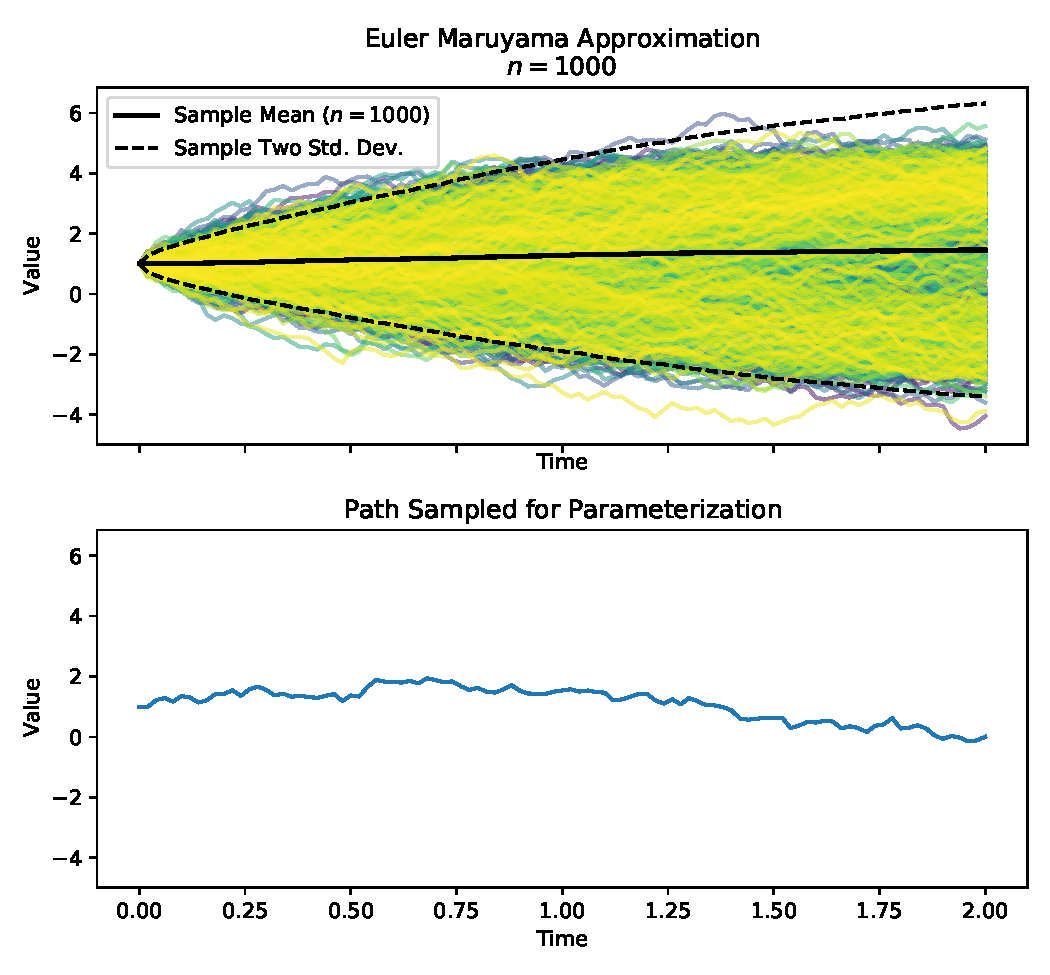
\includegraphics{/Users/macowner/Documents/Stochastic_Calculus/Hmwk_10/hmwk_10_files/figure-latex/plot truth-1.pdf}

\begin{Shaded}
\begin{Highlighting}[]
\NormalTok{sample_time }\OperatorTok{=}\NormalTok{ t_em}
\NormalTok{sample_value }\OperatorTok{=}\NormalTok{ x_em[:, }\DecValTok{1}\NormalTok{].copy()}


\CommentTok{# -- Approximate Likelihood}
\KeywordTok{def}\NormalTok{ approx_ell(theta):}
    \ControlFlowTok{return}\NormalTok{ ell(theta, approx_llh, sample_value, dt, f, g)}


\NormalTok{ml_res }\OperatorTok{=}\NormalTok{ minimize(approx_ell, x0}\OperatorTok{=}\NormalTok{(}\FloatTok{0.5}\NormalTok{, }\DecValTok{3}\NormalTok{), bounds}\OperatorTok{=}\NormalTok{[(}\DecValTok{0}\NormalTok{, }\DecValTok{5}\NormalTok{), (}\DecValTok{0}\NormalTok{, }\DecValTok{5}\NormalTok{)])}

\NormalTok{plt.figure()}
\NormalTok{plot_theta_1 }\OperatorTok{=}\NormalTok{ np.linspace(}\DecValTok{0}\NormalTok{, }\DecValTok{5}\NormalTok{, }\DecValTok{100}\NormalTok{)}
\NormalTok{plot_theta_2 }\OperatorTok{=}\NormalTok{ np.linspace(}\DecValTok{0}\NormalTok{, }\DecValTok{5}\NormalTok{, }\DecValTok{100}\NormalTok{)}
\NormalTok{th_1_xx, th_2_yy }\OperatorTok{=}\NormalTok{ np.meshgrid(plot_theta_1, plot_theta_2)}
\NormalTok{plot_likelihood }\OperatorTok{=}\NormalTok{ np.zeros_like(th_2_yy)}

\ControlFlowTok{for}\NormalTok{ x_idx, th_1 }\KeywordTok{in} \BuiltInTok{enumerate}\NormalTok{(plot_theta_1):}
    \ControlFlowTok{for}\NormalTok{ y_idx, th_2 }\KeywordTok{in} \BuiltInTok{enumerate}\NormalTok{(plot_theta_2):}
\NormalTok{        plot_likelihood[y_idx, x_idx] }\OperatorTok{=}\NormalTok{ approx_ell((th_1, th_2))}

\NormalTok{plt.contour(th_1_xx, th_2_yy, plot_likelihood, levels}\OperatorTok{=}\DecValTok{20}\NormalTok{)}
\end{Highlighting}
\end{Shaded}

\begin{verbatim}
## <matplotlib.contour.QuadContourSet object at 0x1249bb8b0>
\end{verbatim}

\begin{Shaded}
\begin{Highlighting}[]
\NormalTok{plt.xlabel(}\VerbatimStringTok{r'$\textbackslash{}theta_1$'}\NormalTok{)}
\NormalTok{plt.ylabel(}\VerbatimStringTok{r'$\textbackslash{}theta_2$'}\NormalTok{)}
\NormalTok{plt.plot(ml_res.x[}\DecValTok{0}\NormalTok{], ml_res.x[}\DecValTok{1}\NormalTok{], }\StringTok{'ro'}\NormalTok{, label}\OperatorTok{=}\StringTok{'Numerical Min.'}\NormalTok{)}
\NormalTok{plt.plot(THETA_1, THETA_2, }\StringTok{'ko'}\NormalTok{, label}\OperatorTok{=}\StringTok{'Known Parameters'}\NormalTok{)}
\NormalTok{plt.legend()}
\NormalTok{plt.title(}\StringTok{'Likelihood'}\NormalTok{)}
\end{Highlighting}
\end{Shaded}

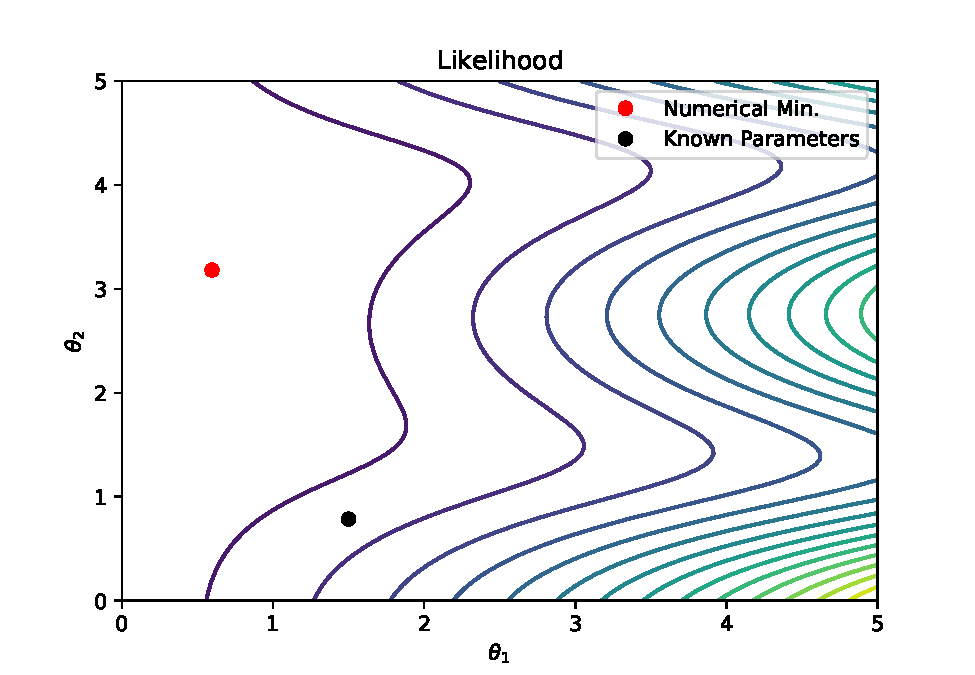
\includegraphics{/Users/macowner/Documents/Stochastic_Calculus/Hmwk_10/hmwk_10_files/figure-latex/show ml method-1.pdf}

\hypertarget{references}{%
\section*{References}\label{references}}
\addcontentsline{toc}{section}{References}

\hypertarget{refs}{}
\leavevmode\hypertarget{ref-sarkka2019applied}{}%
Särkkä, Simo, and Arno Solin. 2019. \emph{Applied Stochastic
Differential Equations}. Vol. 10. Cambridge University Press.


\end{document}
